%% Stand 04. Juli 2026
\subsection{Semivarianz und Variogramm}
\label{KapitelTheorieVariogramm}

Die Semivarianz ist die Größe, mit deren Hilfe die Ähnlichkeit
von zwei Beobachtungen $\mathrm{Z}(s_j)$ und $\mathrm{Z}(s_k)$
eines Zufallsfeldes quantifiziert werden kann und ist dadurch eine wichtige Bestimmungsgröße des Kriging.

\begin{definition} \textbf{Semivarianz} \\
Die \underline{Semivarianz} $\gamma$ eines Zufallsfeldes ist
definiert als die Varianz der Differenz zweier Zufallsvariablen
des Zufallsfelds:
\begin{equation}
\label{Gl_Semivarianz}
\gamma(s_j - s_k) = \frac{1}{2}\mathrm{Var} \left[ \mathrm{Z}(s_j) 
- \mathrm{Z}(s_k)  \right],\ \forall\,s_j,s_k \in \mathcal{S}.
\end{equation}
\end{definition}
\textbf{Anmerkung}: Die Semivarianz gemäß dieser Definition wird 
in der englisch-sprachigen Literatur als \textit{variogram} oder 
auch \textit{semivariogram} bezeichnet. \\
Nun bezeichnet man im deutschen Sprachgebrauch mit 
Variogramm allerdings die grafische Darstellung des Verlaufs 
der Semivarianz, weshalb mit Blick auf eine saubere
Unterscheidung zwischen der Funktion einerseits
und ihrer Darstellung andererseits die Notation Semivarianz für 
die Funktion und Variogramm für ihren Graphen gewählt wurde.\\

Nach den bekannten Rechenregeln für die Varianz von
Zufallsvariablen 
(vgl.\,z.\,B.\,\cite[S.\,102]{Henze2019}) lässt sich  
Gl.\,(\ref{Gl_Semivarianz}) auch schreiben als :
\begin{equation}
\gamma(s_j - s_k) = \frac{1}{2} \left[ 
\mathrm{Var} \left( \mathrm{Z}(s_j) \right) + 
\mathrm{Var} \left( \mathrm{Z}(s_k) \right) \right] - 
\mathrm{Cov} \left( \mathrm{Z}(s_j), \mathrm{Z}(s_k) \right),
\end{equation}
was sich bei Beschränkung auf schwach stationäre Zufallsfelder
unter Nutzung von Gl.\,(\ref{Gl_VarianzZF_schwach_stationär})
weiter vereinfacht zu:
\begin{eqnarray}
\begin{gathered}
\label{Gl_Semivarianz_schwachstationärerFall}
\gamma(s_j - s_k) = \frac{1}{2} \left[ 
\mathrm{Var} \left( \mathrm{Z}(s_j) \right) + 
\mathrm{Var} \left( \mathrm{Z}(s_k) \right) \right] - 
\mathrm{Cov} \left( \mathrm{Z}(s_j), \mathrm{Z}(s_k) \right)=\\
\frac{1}{2} \left[ C(0) + C(0) \right] - C(s_j - s_k) =
\sigma^2 - C(h),\ \textrm{mit } h=(s_j - s_k) \Longleftrightarrow\\
\gamma(h) = \sigma^2 - C(h) = 
\sigma^2\left( 1 - \rho(h)\right),\ \textrm{wobei\ }
\rho(h):= \frac{C(h)}{\sigma^2}.
\end{gathered}
\end{eqnarray}
Die Funktion $\rho(h): \mathbb{R}^d \rightarrow [-1,\,1]$ aus 
Gl.\,(\ref{Gl_Semivarianz_schwachstationärerFall}) 
wird \underline{Korrelations-Funktion} genannt.\\

Damit folgt schließlich im Falle eines isotropen Zufallsfeldes:
\begin{equation}
\label{Gl_Semivarianz_isotroperFall}
\gamma(r) = \sigma^2 - C(r) =
\sigma^2 \left( 1- \rho(r)\right),\ \text{mit\ } r:= \Vert h\Vert. 
\end{equation}

Aus der Kenntnis von zwei der drei Größen Varianz, Kovarianz-Funktion
und Semivarianz eines schwach stationären Zufallsfeldes lässt sich 
also die dritte Größe berechnen.

\subsubsection{Schätzung der empirischen Semivarianz}
\label{KapitelTheorieVariogrammSchätzung}
Unter der Annahme eines isotropen Zufallsfeldes 
gilt für die Semivarianz nach Gl.\,(\ref{Gl_Semivarianz_schwachstationärerFall}):
\begin{eqnarray*}
\begin{gathered}
\gamma(s_j - s_k) = \frac{1}{2}\mathrm{Var} \left[
\mathrm{Z}(s_j) - \mathrm{Z}(s_k)  \right]=
\mathbb{E}\left( \left[ \mathrm{Z}(s_j) - \mathrm{Z}(s_k)
\right]^2 \right) - \left[ \mathbb{E}\left( 
\mathrm{Z}(s_j) - \mathrm{Z}(s_k) \right) \right]^2=\\
\mathbb{E}\left( \left[ \mathrm{Z}(s_j) - \mathrm{Z}(s_k)
\right]^2 \right) -\left( \mu -\mu \right)^2 =
\mathbb{E}\left( \left[ \mathrm{Z}(s_j) - \mathrm{Z}(s_k)
\right]^2 \right)
\end{gathered}
\end{eqnarray*}
womit ein Schätzer für die Semivarianz gegeben ist durch:
\begin{equation}
\label{Gl_Semivarianz_Schätzer_isotroperFall}
\hat{\gamma}(r)= \frac{1}{2\#N(r)} \sum_{j,\,k\, \in N(r)} \left( z(s_j) - z(s_k)\right)^2,
\end{equation}
wobei 
$N(r) = \lbrace (s_j, s_k) : \Vert s_j - s_k\Vert = r 
\wedge s_j,\,s_k \in \mathcal{S}\rbrace$ 
die Menge aller Orte im Gebiet $\mathcal{S}$ mit Abstand $r$
bezeichnet.\\

Falls die Orte $s \in \mathcal{S} \subset \mathbb{R}^d$ der
Zufallsvariablen $\mathrm{Z}(s)$, die gesamthaft das
Zufallsfeld aufbauen können, kontinuierliche Werte annehmen 
(man spricht von geostatistischen Daten), wird die Mächtigkeit 
$\#N(r)$ der Mengen für verschiedene Werte von $r$ typischerweise 
bei Eins oder Null liegen, was zu einem 
\glqq verwackelten\grqq\ Verlauf des
Schätzers $\hat{\gamma}$ der Semivarianz führt.\\

Man verwendet daher in der Praxis das Vorgehen der
 Klasseneinteilung und
partitioniert das Intervall $[0, r_{max}]$ anhand von
Stützstellen $\lbrace r_m\rbrace$ mit 
$0=r_0 < r_1 < \ldots < r_M=r_{max}$ in $M$  
disjunkte Intervalle $R_m=[r_m, r_{m+1}),\ 0 \leq m < M$.\\
Die so definierten Abstandsklassen $\lbrace R_m \rbrace$ werden 
auch als \underline{Lag} bezeichnet\footnote{Deutsche Übersetzungen
haben sich nicht durchgesetzt, weshalb diese Bezeichnung als
Fachbegriff im weiteren Verlauf beibehalten wird.}. \\
Bei der Wahl einer geeigneten Klassenaufteilung sollte beachtet 
werden, dass es für $n$ Datenpunkten einer Beobachtung
maximal $n\cdot(n-1)/2$ paarweise verschiedenen Distanzen gibt.
Die Anzahl der in die Berechnung einbezogenen Datenpunkte sollte 
somit hinreichenden groß sein, um eine aussagekräftige Schätzung zu ermöglichen. \\

Nach dieser Vorarbeit wird dann die Zählung nach 
Gl.\,(\ref{Gl_Semivarianz_Schätzer_isotroperFall}) dahingehend
modifiziert, dass man die Abstände $\Vert s_j - s_k \Vert$ in den 
jeweiligen Klassen betrachtet:
\begin{equation}
\label{Gl_Semivarianz_Schätzer_isotroperFall_Matheron}
\hat{\gamma}(r_m)= \frac{1}{2\#N_m} \sum_{m:\,(s_j-s_k) \in R_m} 
\left( z(s_j) - z(s_k)\right)^2,
\end{equation}
wobei 
$N_m = \lbrace (s_j, s_k) : \Vert s_j - s_k\Vert \in R_m 
\wedge s_j,\,s_k \in \mathcal{S}\rbrace$ die Menge aller Orte 
im Gebiet $\mathcal{S}$ in der Abstands-Klasse $R_m$ bezeichnet.
Der Schätzer gemäß 
Gl.\,(\ref{Gl_Semivarianz_Schätzer_isotroperFall_Matheron})
wird auch \textit{Matheron Semivarianz-Schätzer} 
genannt. \\

Ein weiterer, gängiger 
Semivarianz-Schätzer wurde in 
\cite{Cressie1980} unter Annahme von normal-verteilten 
Zufallsvariablen $\mathrm{X}(s)$ (was auf eine 
$\chi^2$-Verteilung des Ausdrucks ($\mathrm{X}(s_j) - 
\mathrm{X}(s_k))^2$ führt) entwickelt 
und wird daher 
auch \textit{Cressie-Hawkins Semivarianz-Schätzer} genannt:
\begin{equation}
\label{Gl_Semivarianz_Schätzer_isotroperFall_Cressie}
\hat{\gamma}(r_m)= 
\frac{1}
{0.457+ \frac{0.494}{\#N_m} + \frac{0.045}{(\#N_m)^2}} \cdot
\left( \frac{1}{2\#N_m} \sum_{m:\,(s_j-s_k) \in R_m} 
\sqrt{ \vert z(s_j) - z(s_k)\vert }\right)^4
\end{equation}

Es existieren weitere Schätzer für die Semivarianz 
(vgl.\,z.\,B.\,\cite{Dowd1984}, \cite{Genton1998}), die für andere 
unterstellte Eigenschaften des Zufallsfelds die Schätzfunktion optimieren.
Die Vielzahl dieser, an verschiedene Voraussetzungen angepassten Varianten
unterstreicht die eingangs bereits betonte Bedeutung der Semivarianz 
für das Prognoseverfahren des Kriging. \\

Für die Schätzer mit diskretisierten Abständen 
$\lbrace r_m \rbrace$ gibt es für die Festlegung der 
Anzahl $M$ der Klassen und deren jeweiligen Breite 
$(r_{m+1} - r_m)$ keine theoretischen Empfehlungen und ist
daher Teil der operativen Feinabstimmung (vgl.\, hierzu auch 
\cite[S.\,111]{Benndorf2023}).\\

In Abb.\,(\ref{Abb_SemivarianzSchätzung_IsotropesZF_Cressie_und_Matheron}) 
ist beispielhaft ein isotropes Gauß'sches Zufallsfeld und rechts daneben die korrespondierenden Variogramme nach Matheron und Cressie-Hawkins dargestellt.\\

\begin{figure}[H] 
\centering
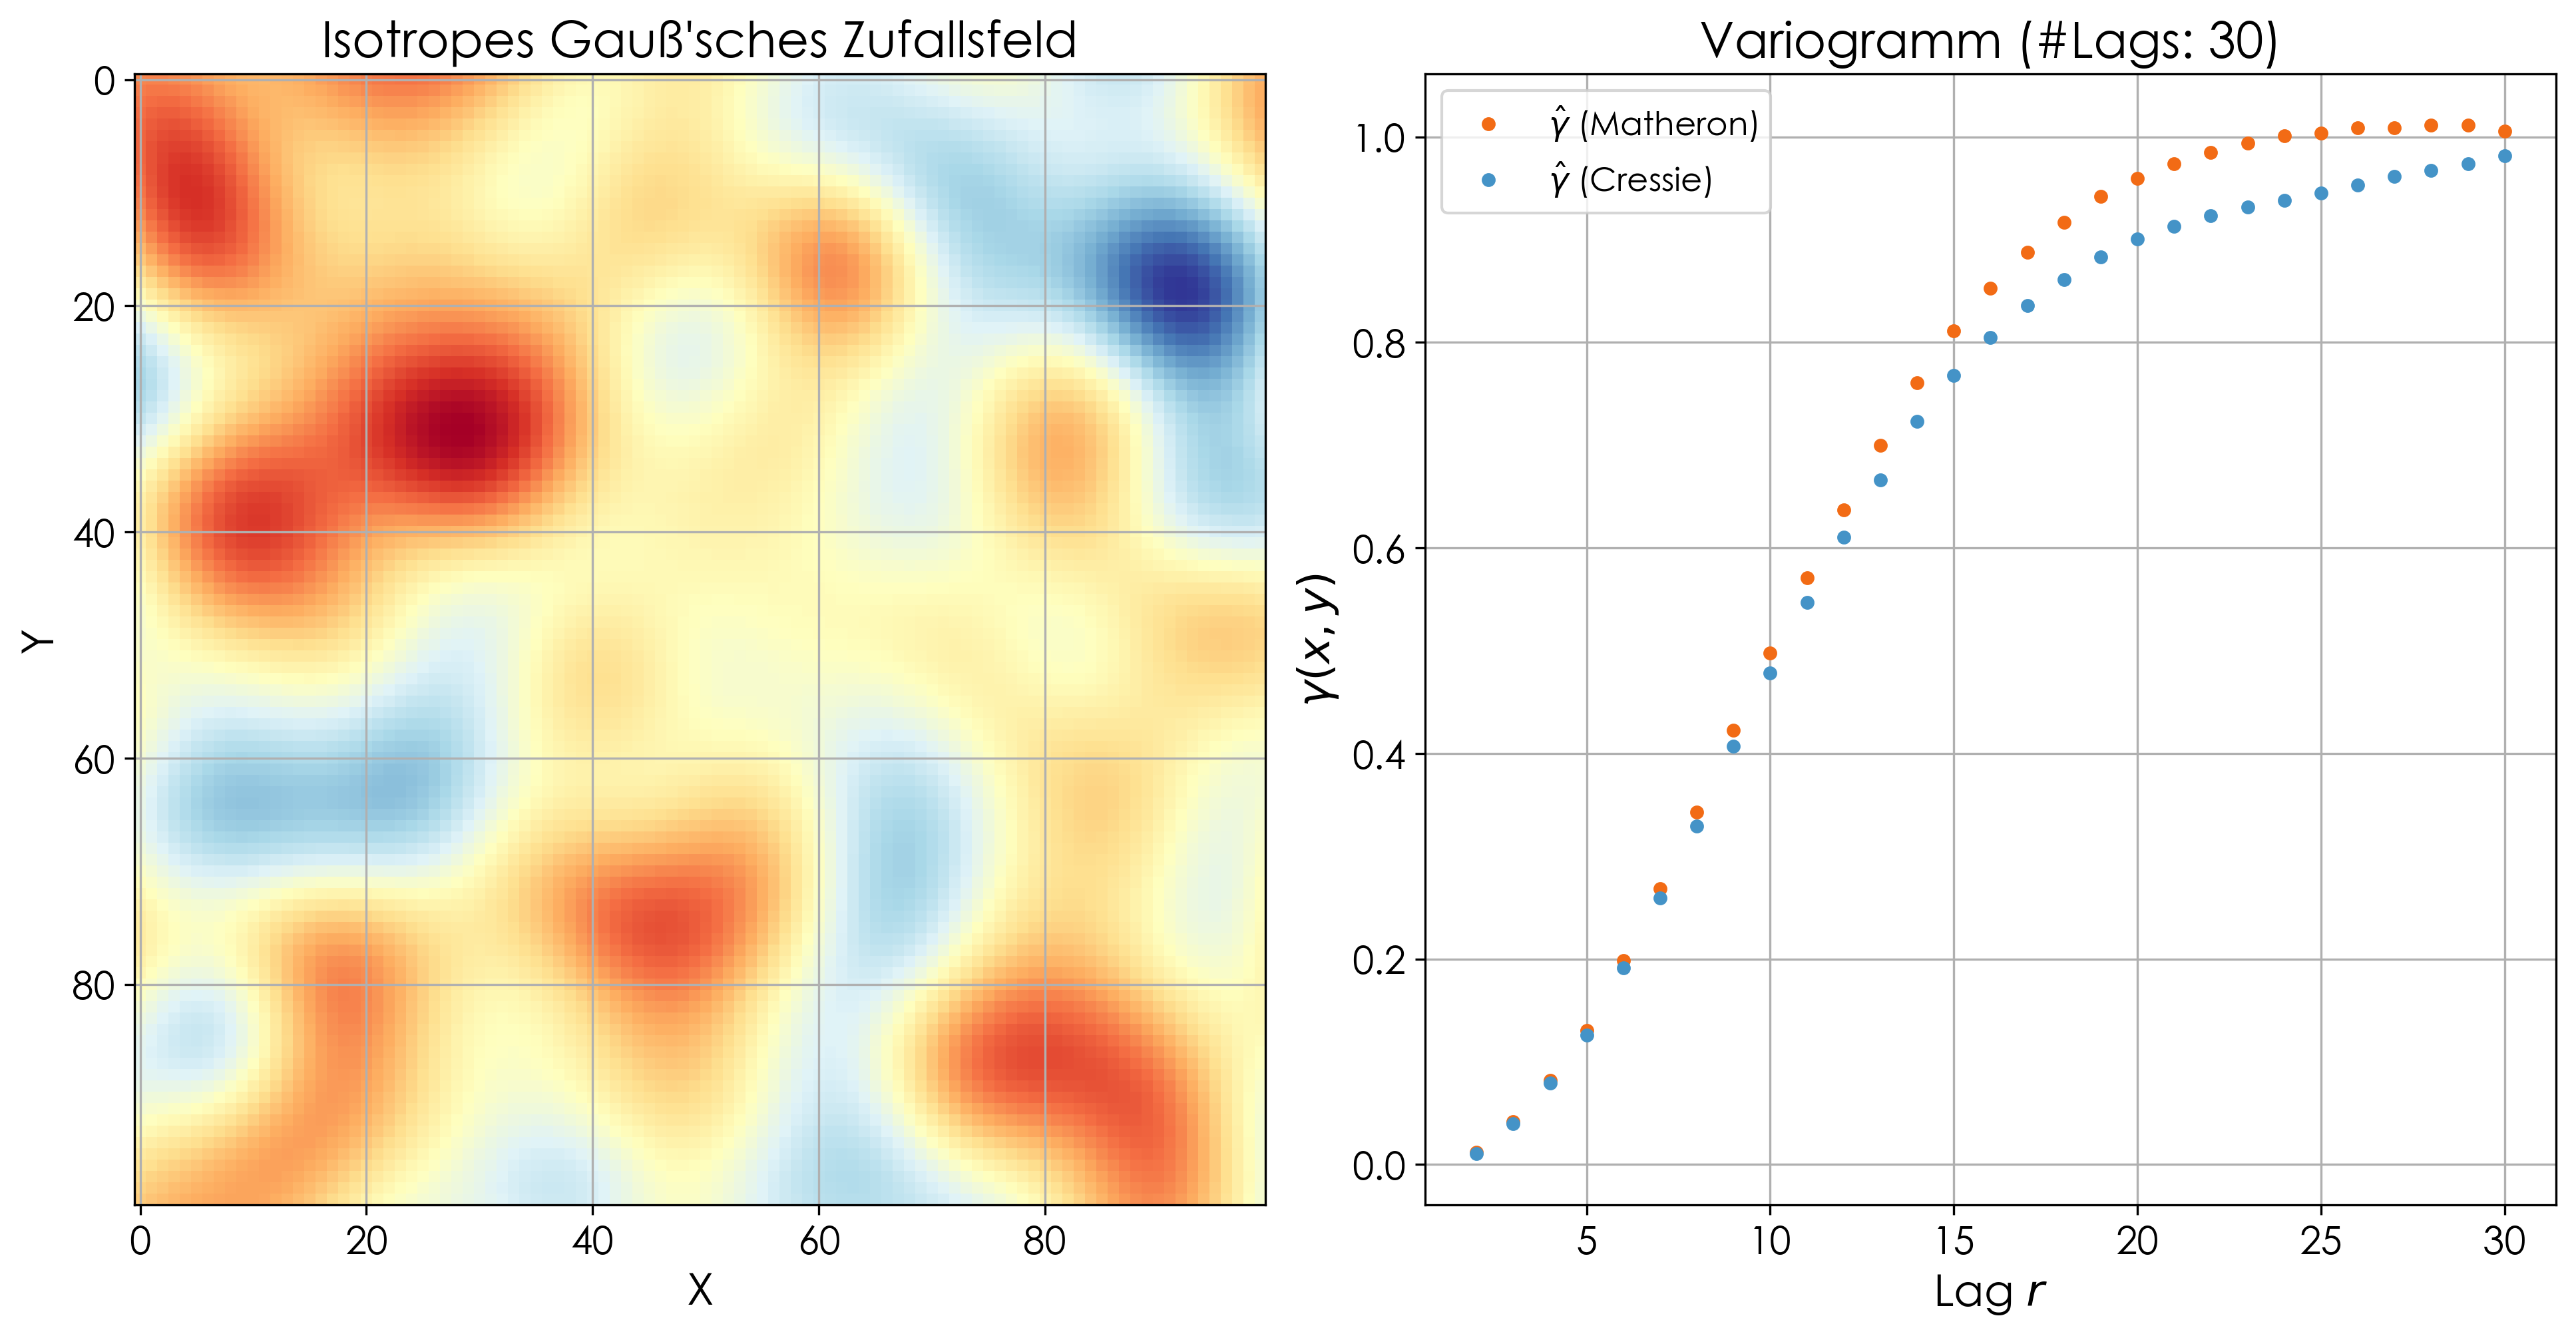
\includegraphics[scale = 0.46]{Bilder/SemivarianzSchätzung_IsotropesZF_Cressie_und_Matheron} 
\caption{\small{Farbkodierte Realisierung $z(x,y)$ eines Gauß'schen Zufallsfelds (links) und 
die korrespondierenden Semivarianz-Schätzfunktionen nach Matheron und Cressie-Hawkins (rechts)}}
\label{Abb_SemivarianzSchätzung_IsotropesZF_Cressie_und_Matheron}
\end{figure} 

Bei der Betrachtung der Variogramme in 
Abb.\,(\ref{Abb_SemivarianzSchätzung_IsotropesZF_Cressie_und_Matheron})
fallen zwei Dinge auf:
\begin{itemize}[topsep=2pt,parsep=1pt,itemsep=0.5pt]
\item[1) ] Mit steigenden Lag $r$ konvergiert die Semivarianz
gegen einen konstanten Wert, der bei dem hier beispielhaft
gewählten Zufallsfeld etwa bei Eins liegt. 
\item[2) ] Der Durchmesser der ähnlich gefärbten Gebiete
innerhalb des Zufallsfeld scheint in etwa mit dem Lag
zusammenzufallen, bei dem die Variogramme eine konstanten Wert
erreichen. Dies erkennt man beispielhaft an dem annähernd
kreisförmigen, rötlich gefärbten Areal 
$(\Delta\,x,\,\Delta\,y) = ([20-40],\,[20-40])$. 
\end{itemize}

Die in diesem Zusammenhang üblichen Fachbegriffe 
werden im nächsten Unterkapitel bereitgestellt, in dem auch 
die Methodik zur Stichproben-Ziehung aus einem Gauß'schen Zufallsfeld 
wie etwa in  
Abb.\,(\ref{Abb_SemivarianzSchätzung_IsotropesZF_Cressie_und_Matheron})
ausgeführt wird. 

\subsection{Kovarianz-Funktionen}
\label{KapitelTheorieKovarianzFunktionen}
Mit der Zielsetzung einer späteren theoretische Beschreibung
ist es hilfreich, die Eigenschaften einer 
Kovarianz-Funktion herauszuarbeiten, wenn für das
korrespondierende Zufallsfeld die Gültigkeit der 
schwachen Stationarität und der Isotropie angenommen werden kann.\\
So lässt sich aus der allgemein gültigen Forderung, dass die
Varianz einer Zufallsvariablen stets größer-gleich Null
sein muss, ableiten, dass die stationäre Kovarianz-Funktion nach
Gl.\,(\ref{Gl_Def_schwach_stationär_Kovarianz}) 
positiv-semidefinit sein muss 
(vgl.\,z.\,B.\,\cite[S.\,55ff]{Webster2007}, 
\cite[S.\,35f]{Journel1989}). \\

Daraus folgen unmittelbar die folgenden Eigenschaften 
einer Kovarianz-Funktion:

\begin{itemize}[topsep=2pt,parsep=1pt,itemsep=0.5pt]
\item[0) ] Kovarianz-Funktionen sind abgeschlossen unter
Addition und Multiplikation; insbesondere sind
Linearkombinationen stationärer Kovarianz-Funktionen
ihrerseits wieder stationäre Kovarianz-Funktionen
(vgl.\,z.\,B.\,\cite[Kap.\,4.2]{Rasmussen2006}, 
\cite[Kap.\,18.2]{Murphy2023}).
\item[1) ] $C(r) = C(-r),\ r \in \mathbb{R}_+$: die 
Kovarianz-Funktion ist eine gerade Funktion.
\item[2) ] $\vert C(r)\vert \leq C(0) = \mathrm{Var} 
\left( \mathrm{Z}(s) \right) = \sigma^2$,
\end{itemize}
die ergänzt werden durch die weitere, theoretisch \textit{nicht} 
notwendige aber praktisch fast immer erfüllte 
\begin{itemize}[topsep=2pt,parsep=1pt,itemsep=0.5pt]
\item[3) ] Eigenschaft 
der räumlich begrenzten Wechselwirkung: $\lim_{r \longrightarrow \infty} C(r) = 0$. Zusammen
 mit Gl.\,(\ref{Gl_Semivarianz_isotroperFall}) folgt damit sofort, 
dass $\lim_{r \longrightarrow \infty} \gamma(r) = \sigma^2$, das heißt,
die Semivarianz konvergiert gegen einen konstanten Wert, 
in Übereinstimmung mit den Beobachtungen, die mit Blick auf 
Abb.\,(\ref{Abb_SemivarianzSchätzung_IsotropesZF_Cressie_und_Matheron}) 
angestellt wurden. 
\end{itemize}  

\vspace*{3pt}
Im folgenden werden einige der theoretischen Modell-Funktionen
aufgeführt, die diesen Rahmenbedingungen für schwach-stationäre
und isotrope Korrelationen gemäß 
Gl.\,(\ref{Gl_Semivarianz_isotroperFall}) genügen und für $\mathcal{S} \subset \mathbb{R}^3$ 
definiert sind.\\

$\circ$ \underline{Sphärisches Modell}
\begin{equation}
\label{Gl_SphärischesModell}
\rho_{sph}(r; \ell) := \left\{\begin{array}{ll} 1- \frac{3}{2} \frac{r}{\ell} 
+ \frac{1}{2}\frac{r^3}{\ell^3}, & \textrm{falls } 0 \leq r < \ell \\
0, & \textrm{falls\ } r \geq \ell \end{array}\right.,\ 
\ell \in \mathbb{R}_+ \setminus \lbrace 0 \rbrace
\end{equation}

\begin{figure}[H] 
\centering

\includegraphics[scale = 0.44]
{TheoModelle_Sphärisch_drei_verschiedene.png} 
\caption{\small{Korrelations-Funktion des 
sphärischen Modells für verschiedene Parameter $\ell$}}
\label{Abb_SphärischesModell_dreiLängen}
\end{figure} 

Aus der Abb.\,(\ref{Abb_SphärischesModell_dreiLängen}) kann man
gut erkennen, dass der Parameter $\ell$ in guter Näherung 
die Distanz $r$ bestimmt, ab der die Korrelations-Funktion auf
Null gefallen ist.\\

Durch die Vorgabe eines Erwartungswerts $\mu$, einer
zwei-dimensionalen Menge $\mathcal{S}$ an Punkten 
und einer Varianz $\sigma^2$ des isotropen, schwach 
stationären Zufallsfeldes, lässt sich für ein konkretes
Korrelations-Modell die Kovarianz-Funktion und damit die Normal-Verteilung eines 
Gauß'schen Zufallsfeld nach 
Gl.\,(\ref{Gl_Def_Gaußfeld_1}) bestimmen. \\
Aus dieser Normal-Verteilung wiederum können Stichproben gezogen
werden (das genaue Vorgehen ist 
z.\,B.\,in \cite{Kroese2015} beschrieben), die 
sich als farbige Fläche darstellen lassen. 
Hierbei wird die Realisierung $z(\tilde{s})$ am Ort 
$\tilde{s}=(\tilde{x}, \tilde{y})$ über eine 
Farbskala kodiert. Diese Vorgehensweise ist im linken 
Teilbild der
Abb.\,(\ref{Abb_SphärischesModell_GRF}) verdeutlicht 
und wird nachfolgend auch für die weiteren, aufgeführten 
Kovarianz-Funktionen angewendet.

\begin{figure}[H] 
\centering

\includegraphics[scale = 0.5]{TheoModelle_Sphärisch_Zufallsfeld.png} 
\caption{\small{Realisierung eines isotropen, schwach stationären
Gauß'schen Zufallsfelds mit sphärischem Modell (links) und das zugehörige Korrelogramm (rechts)}}
\label{Abb_SphärischesModell_GRF}
\end{figure} 

%$\circ$ \underline{Matérn Modell}
%\begin{equation}
%\rho_{mat}(r; \ell, \nu ) := \frac{1}{\Gamma(\nu)2 ^{\nu -1}}
%\left( \frac{\sqrt{2\nu}}{\ell} r \right)^\nu
%\mathrm{K}_\nu \left( \frac{\sqrt{2\nu}}{\ell} r \right),
%\end{equation}
%wobei 
%\begin{itemize}[topsep=2pt,parsep=1pt,itemsep=0.5pt]
%\item[$\bullet$] $\Gamma(\cdot)$ die Gamma-Funktion,
%\item[$\bullet$] $\mathrm{K}_\nu(\cdot)$ die hyperbolische Bessel-Funktion 
%zweiter Art $\rightsquigarrow$ \href{https://en.wikipedia.org/wiki/Bessel_function#Modified_Bessel_functions}
%{Wiki: Bessel function}
%\item[$\bullet$] $\ell,\nu \in \mathbb{R}_+ \setminus \lbrace 0 \rbrace$
% Modell-Parameter
%\end{itemize}
%bezeichnen.\\
%
%\textcolor{red}{Noch zwei, drei Sätze zur
%Bedeutung des Matern Modells}
%
%\begin{figure}[H] 
%\centering
%\includegraphics[scale = 0.44]
%{TheoModelle_Matern_drei_verschiedene.png} 
%\caption{\small{Korrelations-Funktion des 
%Matérn-Modells für verschiedene Parameter $\ell$}}
%\label{Abb_MaternModell_dreiLängen}
%\end{figure} 
%
%\begin{figure}[H] 
%\centering
%
\includegraphics[scale = 0.5]{TheoModelle_Matern_Zufallsfeld.png} 
%\caption{\small{Realisierung eines isotropen, schwach stationären
%Gauß'schen Zufallsfelds mit Matérn Modell (links) und das zugehörige Korrelogramm (rechts)}}
%\label{Abb_MaternModell_GRF}
%\end{figure} 
%
%Im Limes $\nu \rightarrow \infty$
%konvergiert das Matérn Modell gegen das Gauß'sche
%Modell, das heißt, 
%das Gauß'sche Modell ist Teil der Matérn Modell Familie (vgl.\,z.\,B.\,\cite[S.\,84f]{Rasmussen2006}).\\

$\circ$ \underline{Exponentielles Modell}
\begin{equation}
\label{Gl_ExponentiellesModell}
\rho_{exp}(r; \ell) :=  \exp\left( -\frac{r}{\ell} \right),\ 
\ell \in \mathbb{R}_+ \setminus \lbrace 0 \rbrace
\end{equation}

\begin{figure}[H] 
\centering

\includegraphics[scale = 0.44]
{TheoModelle_Exponentiell_drei_verschiedene.png} 
\caption{\small{Korrelations-Funktion des 
exponentiellen Modells für verschiedene Parameter $\ell$}}
\label{Abb_ExponentiellesModell_dreiLängen}
\end{figure} 

\begin{figure}[H] 
\centering

\includegraphics[scale = 0.5]{TheoModelle_Exponentiell_Zufallsfeld.png} 
\caption{\small{Realisierung eines isotropen, schwach stationären
Gauß'schen Zufallsfelds mit exponentiellem Modell (links) und das zugehörige Korrelogramm (rechts)}}
\label{Abb_ExponentiellesModell_GRF}
\end{figure} 

Im Anhang \ref{AnhangWeitereKovarianzFunktionen} 
sind mit dem Stable-, dem Matérn- und dem Gauß'schen
Modell drei weitere der in der Praxis relevante 
Kovarianz-Modelle aufgeführt.\\   

Die obenstehenden Ausführungen zu stationären 
Kovarianz-Funktionen sind beispielsweise auch in 
den Lehrbüchern
\cite[Kap.\,3.5.1]{Montero2015}
\cite[Kap.\,3.3.2]{Oliver2015}, \cite[Kap.\,2.5.1]{Chiles1999},
\cite[Kap.\,4.2.1]{Rasmussen2006} nachzulesen.

\subsubsection{Nugget Effekt}
\label{KapitelTheorieNuggetEffekt}
Im Falle eine schwach stationären Zufallsfeldes folgt aus 
der in Kapitel \ref{KapitelTheorieGrundlagen} hergeleiteten 
Gl.\,(\ref{Gl_Def_schwach_stationär_Kovarianz}), dass 
die Beziehung
\begin{eqnarray}
\begin{gathered}
\gamma(h) = \frac{1}{2} 
\mathrm{Var} \left[ \mathrm{Z}(s+h) - \mathrm{Z}(s) \right] \Longrightarrow \\
\lim_{h \longrightarrow 0} \gamma(h) =0
\end{gathered}
\end{eqnarray}
gilt\footnote{Genau genommen, geht zusätzlich die nicht explizit erwähnte 
Annahme ein, dass für das Zufallsfeld $Z(s)\in \mathcal{L}^2$ erfüllt ist,
wobei $\mathcal{L}^2$ aus allen quadratisch integrierbaren,
messbaren Funktion $f$ besteht, also $\Vert f\Vert_{L^2} < \infty$. 
Details bezüglich der Notation finden sich z.\,B.\,in \cite[Kap.\,12]{Forster2017}.}.\\

Nun kommt es unter realen Bedingungen vor, dass 
\begin{equation}
\label{Gl_Nugget_Effekt}
\lim_{h \longrightarrow 0} \gamma(h) =c_0 > 0
\end{equation}
beobachtet wird, das heißt, es gibt eine Unstetigkeit der Semivarianz
$\gamma(\cdot)$ in der Nähe des Ursprungs.\\
Das Auftreten dieser
Unstetigkeit wird nach \cite[Kap.\,2.7]{Matheron1971} als 
\underline{Nugget-Effekt} und die Sprunghöhe 
$c_0$ in der Gl.\,(\ref{Gl_Nugget_Effekt}) als \underline{Nugget} bezeichnet. \\

Ursächlich für diese Diskontinuität können nach \cite[S.\,51f]{Chiles1999} 
sein:
\begin{itemize}[topsep=2pt,parsep=1pt,itemsep=0.5pt]
\item[$\circ$] eine Mikrostruktur mit einer Reichweite, die kürzer ist als der
Stichprobenträger (beispielsweise der Bohrkopf für Probebohrungen im Bergbauwesen); 
dieser Fall tritt mitunter beim Goldabbau auf und war namensgebend für den Nugget-Effekt 
(vgl.\,z.\,B.\,\cite{Carrasco2010}); 
\item[$\circ$] eine Struktur mit einer Reichweite, die kürzer ist als der 
kleinste technisch mögliche Abstand zwischen den Messpunkten oder
\item[$\circ$] Mess- und Positionierungsfehler.
\end{itemize}

Unabhängig von der genauen Ursache des Nugget-Effekts lässt
sich dieser mathematisch als eine Fallunterscheidung
in den Definitionen der Kovarianz- bzw.\, Korrelations-Funktionen
des Kapitels \ref{KapitelTheorieKovarianzFunktionen} einführen.\\
Beispielsweise würde die Korrelations-Funktion für das 
Gauß'sche Modell nach Gl.\,(\ref{Gl_GaussModell}) durch das Hinzufügen 
eines Nugget-Effekt der Größe $c_0$ wie folgt modifiziert:

\begin{equation}
\label{Gl_GaussModell_mit_Nugget}
\rho_{exp}(r; \ell) := \left\{\begin{array}{ll} 
\exp\left( -\frac{r^2}{\ell^2}\right), & \textrm{falls } r >0\\
c_0, & \textrm{falls\ } r = 0
\end{array}\right.,\ 
\ell \in \mathbb{R}_+ \setminus \lbrace 0 \rbrace
\end{equation}

\vspace*{2mm}
Abb.\,(\ref{Abb_Gauss_mit_ohne_Nugget}) zeigt zwei Realisierungen eines isotropen, 
schwach-stationären Gauß'schen Zufallsfeldes mit
Gauß'scher Korrelations-Funktion einmal mit und einmal ohne Nugget.
Man erkennt deutlich, dass das Einführen eines Nugget-Effekts die auch mit dem bloßen Auge 
erkennbaren Strukturen der Verbundenheit verwässert.

\begin{figure}[H] 
\centering

\includegraphics[width = 0.48\textwidth]{TheoNugget_Gauss_ohne_Nugget.png} 

\includegraphics[width = 0.48\textwidth]{TheoNugget_Gauss_mit_Nugget.png} 
\caption{\small{Realisierung eines isotropen, schwach stationären
Gauß'schen Zufallsfelds mit Gauß'scher Korrelations-Funktion ohne (links) und mit 
Nugget-Effekt (rechts)}}
\label{Abb_Gauss_mit_ohne_Nugget}
\end{figure} 

\subsubsection{Übersicht der eingeführten Fachbegriffe}
In Ergänzung zu
Abb.\,(\ref{Abb_Variogramm_Fachbegriffe}) sind nachfolgend die im 
Kontext der Variogramm-Analyse gängigen Fachbegriffe zusammengefasst:

\begin{figure}[H] 
\centering

\includegraphics[scale = 0.5]{Abb_Variogramm_Fachbegriffe.jpg} 
\caption{\small{Illustration der Fachbegriffe Range, Sill,
Partial Sill und  Nugget in Beziehung zur Semivarianz $\gamma(r)$
 und der Korrelations-Funktion $\rho(r)$}}
\label{Abb_Variogramm_Fachbegriffe}
\end{figure} 

\begin{itemize}[topsep=2pt,parsep=1pt,itemsep=0.5pt]
\item[$\circ$] Der \underline{Range} beschreibt die durchschnittliche 
Reichweite der räumlichen Korrelation. Außerhalb dieser Reichweite 
besteht keine statistische Abhängigkeit der Beobachtungen mehr.
Der Range wird maßgeblich durch den Parameter $\ell$ der in 
Kap.\,\ref{KapitelTheorieKovarianzFunktionen} eingeführten Kovarianz-Modelle 
bestimmt. 
\item[$\circ$] Der \underline{Sill} ist der Grenzwert (das maximale Plateau) den die 
Semivarianz $\gamma(r)$ für unendlich große Abstände erreicht.
\item[$\circ$] Der \underline{Nugget} beschreibt die Unstetigkeit an der Stelle $r=0$ (vgl.\,Kap.\,\ref{KapitelTheorieNuggetEffekt}).
\item[$\circ$] Der \underline{Partial Sill} ist das Plateau, welches durch die 
Differenz (Sill-Nugget) charakterisiert wird.
\end{itemize}










